\paragraph{QuizziPedia::Back-End::App::Models::QuestionModel}
\label{QuizziPedia::Back-End::App::Models::QuestionModel}
\begin{figure}[ht]
	\centering
	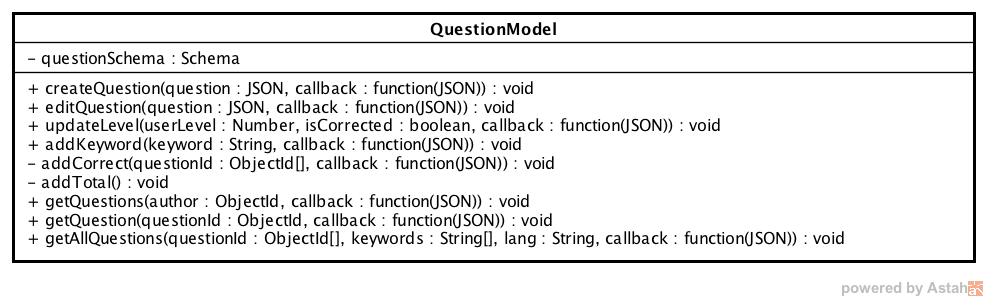
\includegraphics[scale=0.65]{UML/Classi/Back-End/QuizziPedia_Back-End_App_Models_questionModel.png}
	\caption{QuizziPedia::Back-End::App::Models::QuestionModel}
\end{figure}
\FloatBarrier
	\begin{itemize}
		\item \textbf{Descrizione}: classe che modella i dati relativi alle domande all'interno dell'applicazione;	
		\item \textbf{Utilizzo}: viene utilizzata per rappresentare le domande. Si interfaccia alla libreria \\\textit{Mongoose\ped{G}} per la creazione dello schema e dei relativi metodi statici o di istanza;
		\item \textbf{Relazione con altra classi}:
			\begin{itemize}
			\item \textbf{IN \texttt{UserModel}} \\
			Classe che rappresenta tutti gli utenti;
			\item \textbf{OUT \texttt{SummaryModel} }\\
			Classe che rappresenta i riepiloghi dei questionari svolti;
			\item \textbf{OUT \texttt{TopicModel}} \\
			Classe che rappresenta gli argomenti;
			\item \textbf{OUT \texttt{QuizModel}} \\
			Classe che modella i questionari all'interno dell'applicazione;
			\item \textbf{IN \texttt{QuestionController}} \\
			Classe che gestisce la logica applicativa riguardante la visualizzazione, la creazione e la modifica delle domande presenti nell'applicazione;
			\item \textbf{OUT \texttt{UserModel}} \\
			Classe che modella la creazione e la gestione dei dati utente;
			\item \textbf{IN \texttt{QuizModel}} \\
			Classe che modella i questionari all'interno dell'applicazione;
			\item \textbf{OUT \texttt{SummaryModel}} \\
			Classe che modella i riepiloghi all'interno dell'applicazione;
			\item \textbf{IN \texttt{TopicModel}} \\
			Classe che modella gli argomenti all'interno delle domande.
			\end{itemize}
		\item \textbf{Attributi}:
	\begin{itemize}
		\item \texttt{questionSchema: Schema} \\
		Questo campo dati rappresenta lo schema \textit{Mongoose\ped{G}} per le domande e prevede i seguenti attributi:
		\begin{itemize}
			\item \texttt{author: ObjectId}\\ Rappresenta il riferimento all'identificativo nel database dell'utente che ha creato la domanda;
			\item \texttt{makeWith: String}\\ Rappresenta con quale strumento è stata creata la domanda;
			\item \texttt{language: String}\\ Rappresenta la lingua in cui è scritta la domanda; 
			\item \texttt{question: Array<Object>}\\ Array che contiene oggetti di tipo \texttt{JSON}. L'oggetto \texttt{JSON} è rappresentato dai seguenti campi:
				\begin{itemize}
					\item \texttt{type: String}\\ Rappresenta la tipologia di domanda; 
					\item \texttt{questionText: String}\\ Rappresenta il testo della domanda; 
					\item \texttt{image: String}\\ Rappresenta l'\textit{URL\ped{G}} dell'immagine associata al testo della domanda; 
					\item \texttt{answers: Array<Object>}\\ Contiene oggetti di tipo \texttt{JSON}. L'oggetto \texttt{JSON} è rappresentato dai seguenti campi:
					\begin{enumerate}	
										  
						\item \texttt{text: String}\\ Rappresenta il testo della risposta;
        				\item \texttt{url: String}\\ Rappresenta l'immagine della risposta;
        					
        				\item \texttt{isItRight: Boolean}\\ Rappresenta se una risposta è giusta o sbagliata.
        						
	        			\item \texttt{position: Number}\\ Rappresenta quale è la giusta posizione di un testo o immagine all'interno di un esercizio di ordinamento.
        						
        				\item \texttt{text1: String}\\ Rappresenta il primo elemento testuale che deve essere collegato con il secondo elemento testuale o rappresentato da un'immagine;
        				\item \texttt{text2: String}\\ Rappresenta il secondo elemento testuale che deve essere collegato con il primo elemento testuale o rappresentato da un'immagine;
        				\item \texttt{url1: String}\\ Rappresenta il primo elemento rappresentato da un'immagine che deve essere collegato con il secondo elemento testuale o rappresentato da un'immagine;
        				\item \texttt{url2: String}\\ Rappresenta il secondo elemento rappresentato da un'immagine che deve essere collegato con il primo elemento testuale o rappresentato da un immagine.
						
        				\item \texttt{x: Number}\\ Rappresenta la coordinata x di una area cliccabile;
        				\item \texttt{y: Number}\\ Rappresenta la coordinata y di una area cliccabile.  
						
        				\item \texttt{wordNumber: Number}\\ Rappresenta la posizione dello spazio vuoto in cui deve andare inserita la parola.      						  						
					\end{enumerate}
				\end{itemize}			
			\item \texttt{keywords: Array<String>}\\ Contiene oggetti di tipo \texttt{String} che rappresentano le parole chiave utili per ricercare una domanda;	 
			\item \texttt{level: Number}\\ Rappresenta la difficoltà della domanda;
			\item \texttt{totalAnswers: Number}\\ Rappresenta le risposte totali che tutti gli utenti hanno dato alla domanda;
			\item \texttt{correctAnswers: Number}\\ Rappresenta quante risposte corrette hanno dato gli utenti che hanno risposto alla domanda.
		
		\end{itemize}
	\end{itemize}
\item \textbf{Metodi}:
	\begin{itemize}
	\item \texttt{+ createQuestion(question: JSON, callback: function(JSON)): void} \\
	Metodo che permette la creazione di una nuova domanda. \\
		\textbf{Parametri}:
		\begin{itemize}
			\item \texttt{question: JSON} \\
			Rappresenta le informazioni che andranno a comporre la domanda da creare;
			\item \texttt{callback: function(JSON)} \\
			Rappresenta la \textit{callback\ped{G}} che verrà eseguita al termine dell'elaborazione nel caso non si verifichino errori durante l'esecuzione;
		\end{itemize}   
	\item \texttt{+ editQuestion(question: JSON, callback: function(JSON)): void} \\
	Metodo che permette di modificare una domanda già esistente. \\
		\textbf{Parametri}:
		\begin{itemize}
			\item \texttt{question : JSON} \\
			Rappresenta le nuove informazioni che andranno a modificare le informazioni precedenti di una specifica domanda;
			\item \texttt{callback: function(JSON)} \\
			Rappresenta la \textit{callback\ped{G}} che verrà eseguita al termine dell'elaborazione del metodo in caso non si verifichino errori durante l'esecuzione;
		\end{itemize}
	\item \texttt{+ getQuestions(author:ObjectId, callback: function(JSON)): void} \\
	Metodo che permette di ottenere una lista domanda già esistente in relazione ad un autore predefinito. \\
		\textbf{Parametri}:
		\begin{itemize}
			\item \texttt{author : ObjectId} \\
			Rappresenta l'autore delle domande;
			\item \texttt{callback: function(JSON)} \\
			Rappresenta la \textit{callback\ped{G}} che verrà eseguita al termine dell'elaborazione del metodo in caso non si verifichino errori durante l'esecuzione;
		\end{itemize}
	\item \texttt{+ getQuestion(questionId: ObjectId, callback: function(JSON)): void} \\
	Metodo che permette di ottenere una determinata domanda a partire dall'id della domanda passata. \\
			\textbf{Parametri}:
			\begin{itemize}
				\item \texttt{questionId: ObjectId} \\
				Rappresenta l'id della domanda da andare a cercare;
				\item \texttt{callback: function(JSON)} \\
				Rappresenta la \textit{callback\ped{G}} che verrà eseguita al termine dell'elaborazione del metodo in caso non si verifichino errori durante l'esecuzione;
			\end{itemize}	
			
	\item \texttt{+ getAllQuestions(questionId: ObjectId[], keywords:String[], lang:String, callback: function(JSON)): void} \\
	Metodo che permette di ottenere una array di domande a partire da: un array di riferimenti delle domande passate, un'array di keywords e una lingua. \\
		\textbf{Parametri}:
		\begin{itemize}
			\item \texttt{questionId: ObjectId[]} \\
			Rappresenta un'array di riferimenti delle domande passate;
			\item \texttt{keywords: String[]} \\
			Rappresenta un'array di keywords;
			\item \texttt{lang: String} \\
			Rappresenta una determinata lingua;
			\item \texttt{callback: function(JSON)} \\
			Rappresenta la \textit{callback\ped{G}} che verrà eseguita al termine dell'elaborazione del metodo in caso non si verifichino errori durante l'esecuzione;
		\end{itemize}	
		
	\item \texttt{+ addKeyword(keyword: String, callback: function(JSON)): void} \\
	Metodo che permette di aggiungere delle parole chiave ad una specifica domanda. \\
		\textbf{Parametri}:
			 \begin{itemize}
			 	\item \texttt{keyword: String} \\
			 	Rappresenta la parola chiave da inserire;
			 	\item \texttt{callback: function(JSON)} \\
			 	Rappresenta la \textit{callback\ped{G}} che verrà eseguita al termine dell'elaborazione del metodo in caso si verifichino errori durante l'esecuzione;
			 \end{itemize}
	\item \texttt{+ updateLevel(userLevel: Number, isCorrected: boolean): void} \\
	Metodo che permette di aggiornare il livello di difficoltà della domanda, questo metodo è chiamato ogni qualvolta un utente risponde ad una domanda durante un allenamento.\\
		\textbf{Parametri}:
			\begin{itemize}
				\item \texttt{userLevel: Number} \\
				Indica, con un numero compreso tra 1 e 1000, l'abilità dell'utente che ha risposto alla domanda;
				\item \texttt{isCorrected: boolean} \\
				Indica se l'utente che ha risposto alla domanda ha risposto correttamente.
			\end{itemize}  
	\item \texttt{- addCorrect(questionId: ObjectId[], callback: function(JSON)): void} \\
	Metodo che permette di incrementare il contatore di risposte corrette di una determinata domanda;
		\textbf{Parametri}:
			\begin{itemize}
				\item \texttt{questionId: ObjectId[]} \\
					Rappresenta un'array di riferimenti delle domande passate;
				\item \texttt{callback: function(JSON)} \\
					Rappresenta la \textit{callback\ped{G}} che verrà eseguita al termine dell'elaborazione del metodo in caso si verifichino errori durante l'esecuzione;
			\end{itemize}
	\item \texttt{- addTotal(questionId: ObjectId[], callback: function(JSON)): void} \\
	Metodo che permette di incrementare il contatore delle risposte date di una determinata domanda;
		\textbf{Parametri}:
			\begin{itemize}
				\item \texttt{questionId: ObjectId[]} \\
				Rappresenta un'array di riferimenti delle domande passate;
				\item \texttt{callback: function(JSON)} \\
				Rappresenta la \textit{callback\ped{G}} che verrà eseguita al termine dell'elaborazione del metodo in caso si verifichino errori durante l'esecuzione;
			\end{itemize}
	\end{itemize}
\end{itemize}
